\documentclass{article}

\usepackage{amsmath}
\usepackage{amssymb}
\usepackage{amsthm}
\usepackage{mathtext}
\usepackage{mathtools}
\usepackage[T1,T2A]{fontenc}
\usepackage[utf8]{inputenc}
\usepackage[left=2cm,right=2cm,top=2cm,bottom=2cm]{geometry}
\usepackage{microtype}
\usepackage{enumitem}
\usepackage{bm}
\usepackage{cancel}
\usepackage{proof}
\usepackage{epigraph}
\usepackage{titlesec}
\usepackage[dvipsnames]{xcolor}
\usepackage{stmaryrd}
\usepackage{cellspace}
\usepackage{cmll}
\usepackage{multirow}
\usepackage{booktabs}
\usepackage{tikz}
\usepackage{caption}
\usepackage{wrapfig}
\usepackage{minted}
\usepackage{svg}

\usepackage[hidelinks]{hyperref}

\usepackage[russian]{babel}
\selectlanguage{russian}

\hypersetup{%
    colorlinks=true,
    linkcolor=blue
}

%\pagenumbering{gobble}

\title{Домашнее задание по теории кодирования}
\author{Артем Оганджанян, M3439, вариант 49}
\date{}

\begin{document}

\maketitle

\section{\texorpdfstring{Глава 2}{Section 2}}
\[
    H =
    \begin{pmatrix}
        0 & 1 & 0 & 1 & 0 & 0 & 1 & 1 & 1 & 1 \\
        1 & 0 & 1 & 1 & 1 & 0 & 1 & 0 & 0 & 1 \\
        0 & 1 & 1 & 1 & 1 & 1 & 0 & 0 & 1 & 1 \\
        1 & 0 & 0 & 1 & 1 & 0 & 1 & 0 & 1 & 0
    \end{pmatrix}
\]
\subsection{\texorpdfstring{Задача 3}{Task 3}}
Поменяем местами 6-ой и 7-ой столбцы, чтобы последние 4 столбца были ЛНЗ.
\[
    H' =
    \begin{pmatrix}
        0 & 1 & 0 & 1 & 0 & 1 & 0 & 1 & 1 & 1 \\
        1 & 0 & 1 & 1 & 1 & 1 & 0 & 0 & 0 & 1 \\
        0 & 1 & 1 & 1 & 1 & 0 & 1 & 0 & 1 & 1 \\
        1 & 0 & 0 & 1 & 1 & 1 & 0 & 0 & 1 & 0
    \end{pmatrix}
\]
Приведём её к виду $H' = (P^T\ I_4)$.
\begin{align*}
    &\begin{pmatrix}
        0 & 1 & 0 & 1 & 0 & 1 & 0 & 1 & 1 & 1 \\
        1 & 0 & 1 & 1 & 1 & 1 & 0 & 0 & 0 & 1 \\
        0 & 1 & 1 & 1 & 1 & 0 & 1 & 0 & 1 & 1 \\
        1 & 0 & 0 & 1 & 1 & 1 & 0 & 0 & 1 & 0
    \end{pmatrix}
    \xrightarrow{1\coloneqq1+3}
    &&\begin{pmatrix}
        0 & 0 & 1 & 0 & 1 & 1 & 1 & 1 & 0 & 0 \\
        1 & 0 & 1 & 1 & 1 & 1 & 0 & 0 & 0 & 1 \\
        0 & 1 & 1 & 1 & 1 & 0 & 1 & 0 & 1 & 1 \\
        1 & 0 & 0 & 1 & 1 & 1 & 0 & 0 & 1 & 0
    \end{pmatrix}
    \xrightarrow{2\coloneqq1+2+3}\\
    &\begin{pmatrix}
        0 & 0 & 1 & 0 & 1 & 1 & 1 & 1 & 0 & 0 \\
        1 & 1 & 1 & 0 & 1 & 0 & 0 & 1 & 1 & 0 \\
        0 & 1 & 1 & 1 & 1 & 0 & 1 & 0 & 1 & 1 \\
        1 & 0 & 0 & 1 & 1 & 1 & 0 & 0 & 1 & 0
    \end{pmatrix}
    \xrightarrow{3\coloneqq1+2+3+4}
    &&\begin{pmatrix}
        0 & 0 & 1 & 0 & 1 & 1 & 1 & 1 & 0 & 0 \\
        1 & 1 & 1 & 0 & 1 & 0 & 0 & 1 & 1 & 0 \\
        0 & 0 & 1 & 0 & 0 & 0 & 0 & 0 & 1 & 1 \\
        1 & 0 & 0 & 1 & 1 & 1 & 0 & 0 & 1 & 0
    \end{pmatrix}
    \xrightarrow{4\coloneqq3+4}\\
    &\begin{pmatrix}
        0 & 0 & 1 & 0 & 1 & 1 & 1 & 1 & 0 & 0 \\
        1 & 1 & 1 & 0 & 1 & 0 & 0 & 1 & 1 & 0 \\
        0 & 0 & 1 & 0 & 0 & 0 & 0 & 0 & 1 & 1 \\
        1 & 0 & 1 & 1 & 1 & 1 & 0 & 0 & 0 & 1
    \end{pmatrix}
    \xrightarrow{3\coloneqq3+4}
    &&\begin{pmatrix}
        0 & 0 & 1 & 0 & 1 & 1 & 1 & 1 & 0 & 0 \\
        1 & 1 & 1 & 0 & 1 & 0 & 0 & 1 & 1 & 0 \\
        1 & 0 & 0 & 1 & 1 & 1 & 0 & 0 & 1 & 0 \\
        1 & 0 & 1 & 1 & 1 & 1 & 0 & 0 & 0 & 1
    \end{pmatrix}
    \xrightarrow{2\coloneqq2+3}\\
    &\begin{pmatrix}
        0 & 0 & 1 & 0 & 1 & 1 & 1 & 1 & 0 & 0 \\
        0 & 1 & 1 & 1 & 0 & 1 & 0 & 1 & 0 & 0 \\
        1 & 0 & 0 & 1 & 1 & 1 & 0 & 0 & 1 & 0 \\
        1 & 0 & 1 & 1 & 1 & 1 & 0 & 0 & 0 & 1
    \end{pmatrix}
    \xrightarrow{1\coloneqq1+2}\
    &&\begin{pmatrix}
        0 & 1 & 0 & 1 & 1 & 0 & 1 & 0 & 0 & 0 \\
        0 & 1 & 1 & 1 & 0 & 1 & 0 & 1 & 0 & 0 \\
        1 & 0 & 0 & 1 & 1 & 1 & 0 & 0 & 1 & 0 \\
        1 & 0 & 1 & 1 & 1 & 1 & 0 & 0 & 0 & 1
    \end{pmatrix}
\end{align*}
Получаем
\[
    G' =
    \begin{pmatrix}
        1 & 0 & 0 & 0 & 0 & 0 & 0 & 0 & 1 & 1 \\
        0 & 1 & 0 & 0 & 0 & 0 & 1 & 1 & 0 & 0 \\
        0 & 0 & 1 & 0 & 0 & 0 & 0 & 1 & 0 & 1 \\
        0 & 0 & 0 & 1 & 0 & 0 & 1 & 1 & 1 & 1 \\
        0 & 0 & 0 & 0 & 1 & 0 & 1 & 0 & 1 & 1 \\
        0 & 0 & 0 & 0 & 0 & 1 & 0 & 1 & 1 & 1 \\
    \end{pmatrix}
    \quad
    \xRightarrow[~6\coloneqq7~]{~7\coloneqq6~}
    \quad
    G =
    \begin{pmatrix}
        1 & 0 & 0 & 0 & 0 & 0 & 0 & 0 & 1 & 1 \\
        0 & 1 & 0 & 0 & 0 & 1 & 0 & 1 & 0 & 0 \\
        0 & 0 & 1 & 0 & 0 & 0 & 0 & 1 & 0 & 1 \\
        0 & 0 & 0 & 1 & 0 & 1 & 0 & 1 & 1 & 1 \\
        0 & 0 & 0 & 0 & 1 & 1 & 0 & 0 & 1 & 1 \\
        0 & 0 & 0 & 0 & 0 & 0 & 1 & 1 & 1 & 1 \\
    \end{pmatrix}
    \text{.}
\]
$n = 10$, $k = 6$, скорость $R=\frac{6}{10}=0.6=\frac{3}{5}$.

Несложно проверить, что любые два столбца матрицы $H$ ЛНЗ, то есть в сумме дают
ненулевой вектор, то есть все столбцы различны.
В то же время, первый, второй и четвёртый столбцы в сумме дают нулевой вектор.
По теореме 2.4 это означает, что минимальное расстояние кода с проверочной
матрицей $H$ равно трём.

\subsection{\texorpdfstring{Задача 7}{Task 7}}
\begin{table}[h]
    \centering
    \begin{tabular}{c c} \toprule
        Синдром & Вектор ошибок \\ \midrule
        $\begin{pmatrix}0&0&0&1\end{pmatrix}$&$\begin{pmatrix}0&0&0&1&0&0&0&0&0&1\end{pmatrix}$\\
        $\begin{pmatrix}0&0&1&0\end{pmatrix}$&$\begin{pmatrix}0&0&0&0&0&1&0&0&0&0\end{pmatrix}$\\
        $\begin{pmatrix}0&0&1&1\end{pmatrix}$&$\begin{pmatrix}0&0&0&0&0&0&0&1&1&0\end{pmatrix}$\\
        $\begin{pmatrix}0&1&0&0\end{pmatrix}$&$\begin{pmatrix}0&0&0&1&0&0&0&0&1&0\end{pmatrix}$\\
        $\begin{pmatrix}0&1&0&1\end{pmatrix}$&$\begin{pmatrix}1&0&0&0&0&0&0&0&0&0\end{pmatrix}$\\
        $\begin{pmatrix}0&1&1&0\end{pmatrix}$&$\begin{pmatrix}0&0&1&0&0&0&0&0&0&0\end{pmatrix}$\\
        $\begin{pmatrix}0&1&1&1\end{pmatrix}$&$\begin{pmatrix}0&0&0&0&1&0&0&0&0&0\end{pmatrix}$\\
        $\begin{pmatrix}1&0&0&0\end{pmatrix}$&$\begin{pmatrix}0&0&0&0&0&0&0&1&0&0\end{pmatrix}$\\
        $\begin{pmatrix}1&0&0&1\end{pmatrix}$&$\begin{pmatrix}0&0&0&0&0&1&0&0&1&0\end{pmatrix}$\\
        $\begin{pmatrix}1&0&1&0\end{pmatrix}$&$\begin{pmatrix}0&1&0&0&0&0&0&0&0&0\end{pmatrix}$\\
        $\begin{pmatrix}1&0&1&1\end{pmatrix}$&$\begin{pmatrix}0&0&0&0&0&0&0&0&1&0\end{pmatrix}$\\
        $\begin{pmatrix}1&1&0&0\end{pmatrix}$&$\begin{pmatrix}0&0&0&0&0&1&0&0&0&1\end{pmatrix}$\\
        $\begin{pmatrix}1&1&0&1\end{pmatrix}$&$\begin{pmatrix}0&0&0&0&0&0&1&0&0&0\end{pmatrix}$\\
        $\begin{pmatrix}1&1&1&0\end{pmatrix}$&$\begin{pmatrix}0&0&0&0&0&0&0&0&0&1\end{pmatrix}$\\
        $\begin{pmatrix}1&1&1&1\end{pmatrix}$&$\begin{pmatrix}0&0&0&1&0&0&0&0&0&0\end{pmatrix}$\\ \bottomrule
    \end{tabular}
    \caption{Таблица синдромного декодирования.}
\end{table}
Код:
\inputminted[linenos]{python}{../../code/ch2/syndec.py}

\section{\texorpdfstring{Глава 3}{Section 3}}
$n = 24$, $k = 12$, $d = 8$.
Граница Хэминга:
\[
    2^k \leq \frac{2^n}{\sum_{i=0}^t C_n^i} \text{, где } d \geq 2t + 1\text{.}
\]
Граница Варшамова-Гильберта:
\[
    2^{n-k} > \sum_{i=0}^{d-2} C_{n-1}^i\text{.}
\]
Граница Грайсмера:
\[
    n \geq \sum_{i=0}^{k-1} \left\lceil \frac{d}{2^i} \right\rceil\text{.}
\]

\subsection{\texorpdfstring{Задача 3}{Task 3}}
Граница Хэминга:
\[
    \sum_{i=0}^3 C_{24}^i \leq 2^{24-k} \implies 2325 \leq 2^{24-k} \implies
    2^k \leq \frac{2^{24}}{2325} \implies k \leq 12\text{.}
\]
Граница Варшамова-Гильберта:
\[
    2^{24-k} > \sum_{i=0}^6 C_{23}^i \implies 2^{24-k} > 145499 \implies
    2^k < \frac{2^{24}}{145499} \implies k \leq 6\text{.}
\]
Проверим $k \in [7..12]$ с помощью границы Грайсмера:
\begin{center}
    \begin{tabular}{c c}
        \toprule
        $k$ & $\min n$ \\ \midrule
        7  & 18 \\
        8  & 19 \\
        9  & 20 \\
        10 & 21 \\
        11 & 22 \\
        12 & 23 \\ \bottomrule
    \end{tabular}
\end{center}
Все $k$ в промежутке удовлетворяют границе Грайсмера.
Получаем, что $k \leq 12$.

\subsection{\texorpdfstring{Задача 4}{Task 4}}
Граница Хэминга:
\[
    2^{12} \leq \frac{2^{24}}{\sum_{i=0}^t C_{24}^i} \implies
    \sum_{i=0}^t C_{24}^i \leq 2^{12} \implies
    t_{\max} = 3 \implies d \leq 8 \text{.}
\]
Граница Варшамова-Гильберта:
\[
    2^{n-k} = 2^{12} > \sum_{i=0}^{d-2} C_{23}^i \implies d \leq 5\text{.}
\]
Проверим $d \in [6..8]$ с помощью границы Грайсмера:
\begin{center}
    \begin{tabular}{c c}
        \toprule
        $d$ & $\min n$ \\ \midrule
        6 & 20 \\
        7 & 22 \\
        8 & 23 \\ \bottomrule
    \end{tabular}
\end{center}
Все $d$ в промежутке удовлетворяют границе Грайсмера.
Получаем, что $d \leq 8$.

\section{\texorpdfstring{Глава 4}{Section 4}}
\[
    H =
    \begin{pmatrix}
        0 & 1 & 0 & 1 & 0 & 0 & 1 & 1 & 1 & 1 \\
        1 & 0 & 1 & 1 & 1 & 0 & 1 & 0 & 0 & 1 \\
        0 & 1 & 1 & 1 & 1 & 1 & 0 & 0 & 1 & 1 \\
        1 & 0 & 0 & 1 & 1 & 0 & 1 & 0 & 1 & 0
    \end{pmatrix}
\]
Приведём матрицу к МСФ:
\[
    H' =
    \begin{pmatrix}
        1&1&1&0&1&0&0&1&1&0\\
        0&1&0&1&1&1&0&0&0&0\\
        0&0&1&0&1&1&1&1&0&0\\
        0&0&0&0&1&1&1&1&1&1
    \end{pmatrix}
\]

\begin{figure}[p]
    \centering
    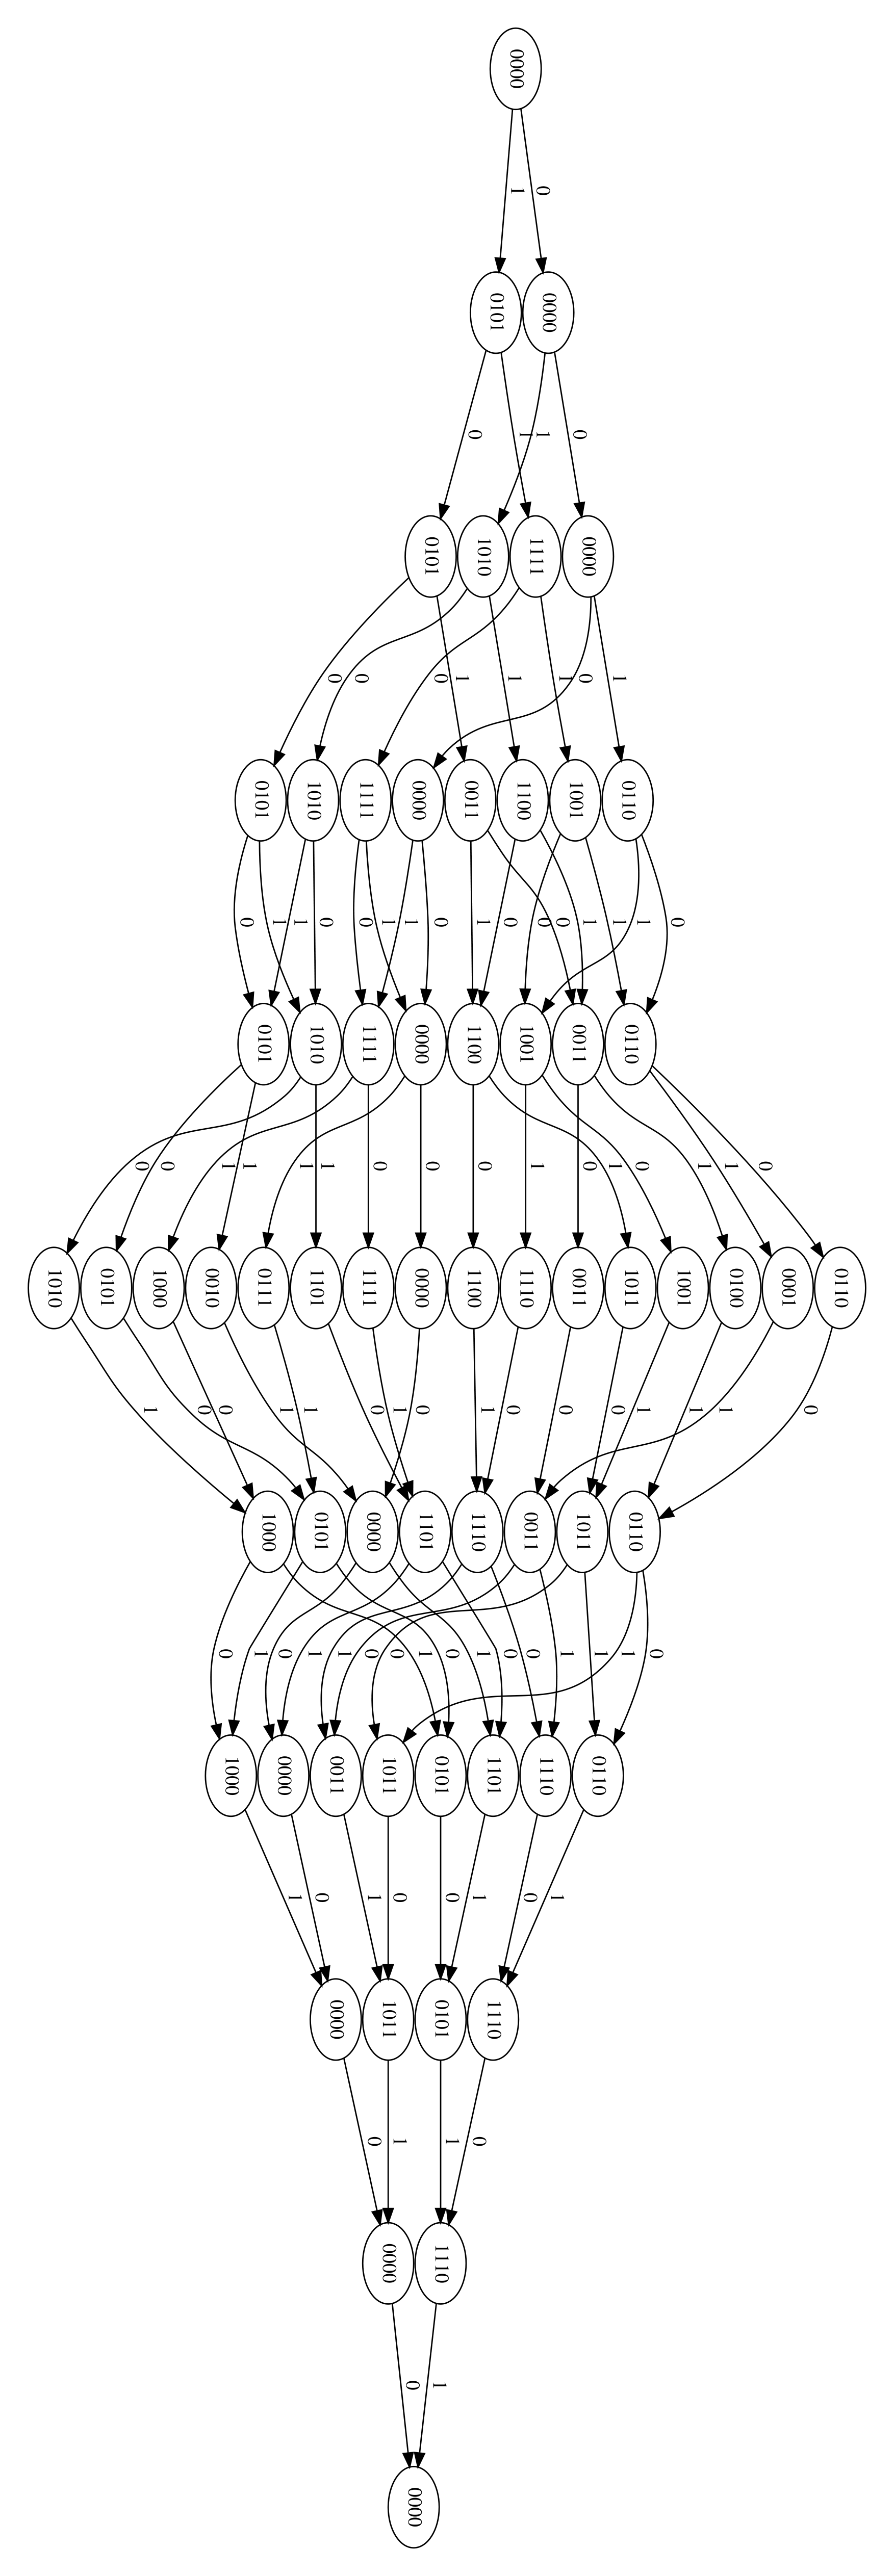
\includegraphics[height=0.95\textheight]{h.png}
    \caption{Синдромная решётка.}
\end{figure}
\begin{figure}[p]
    \centering
    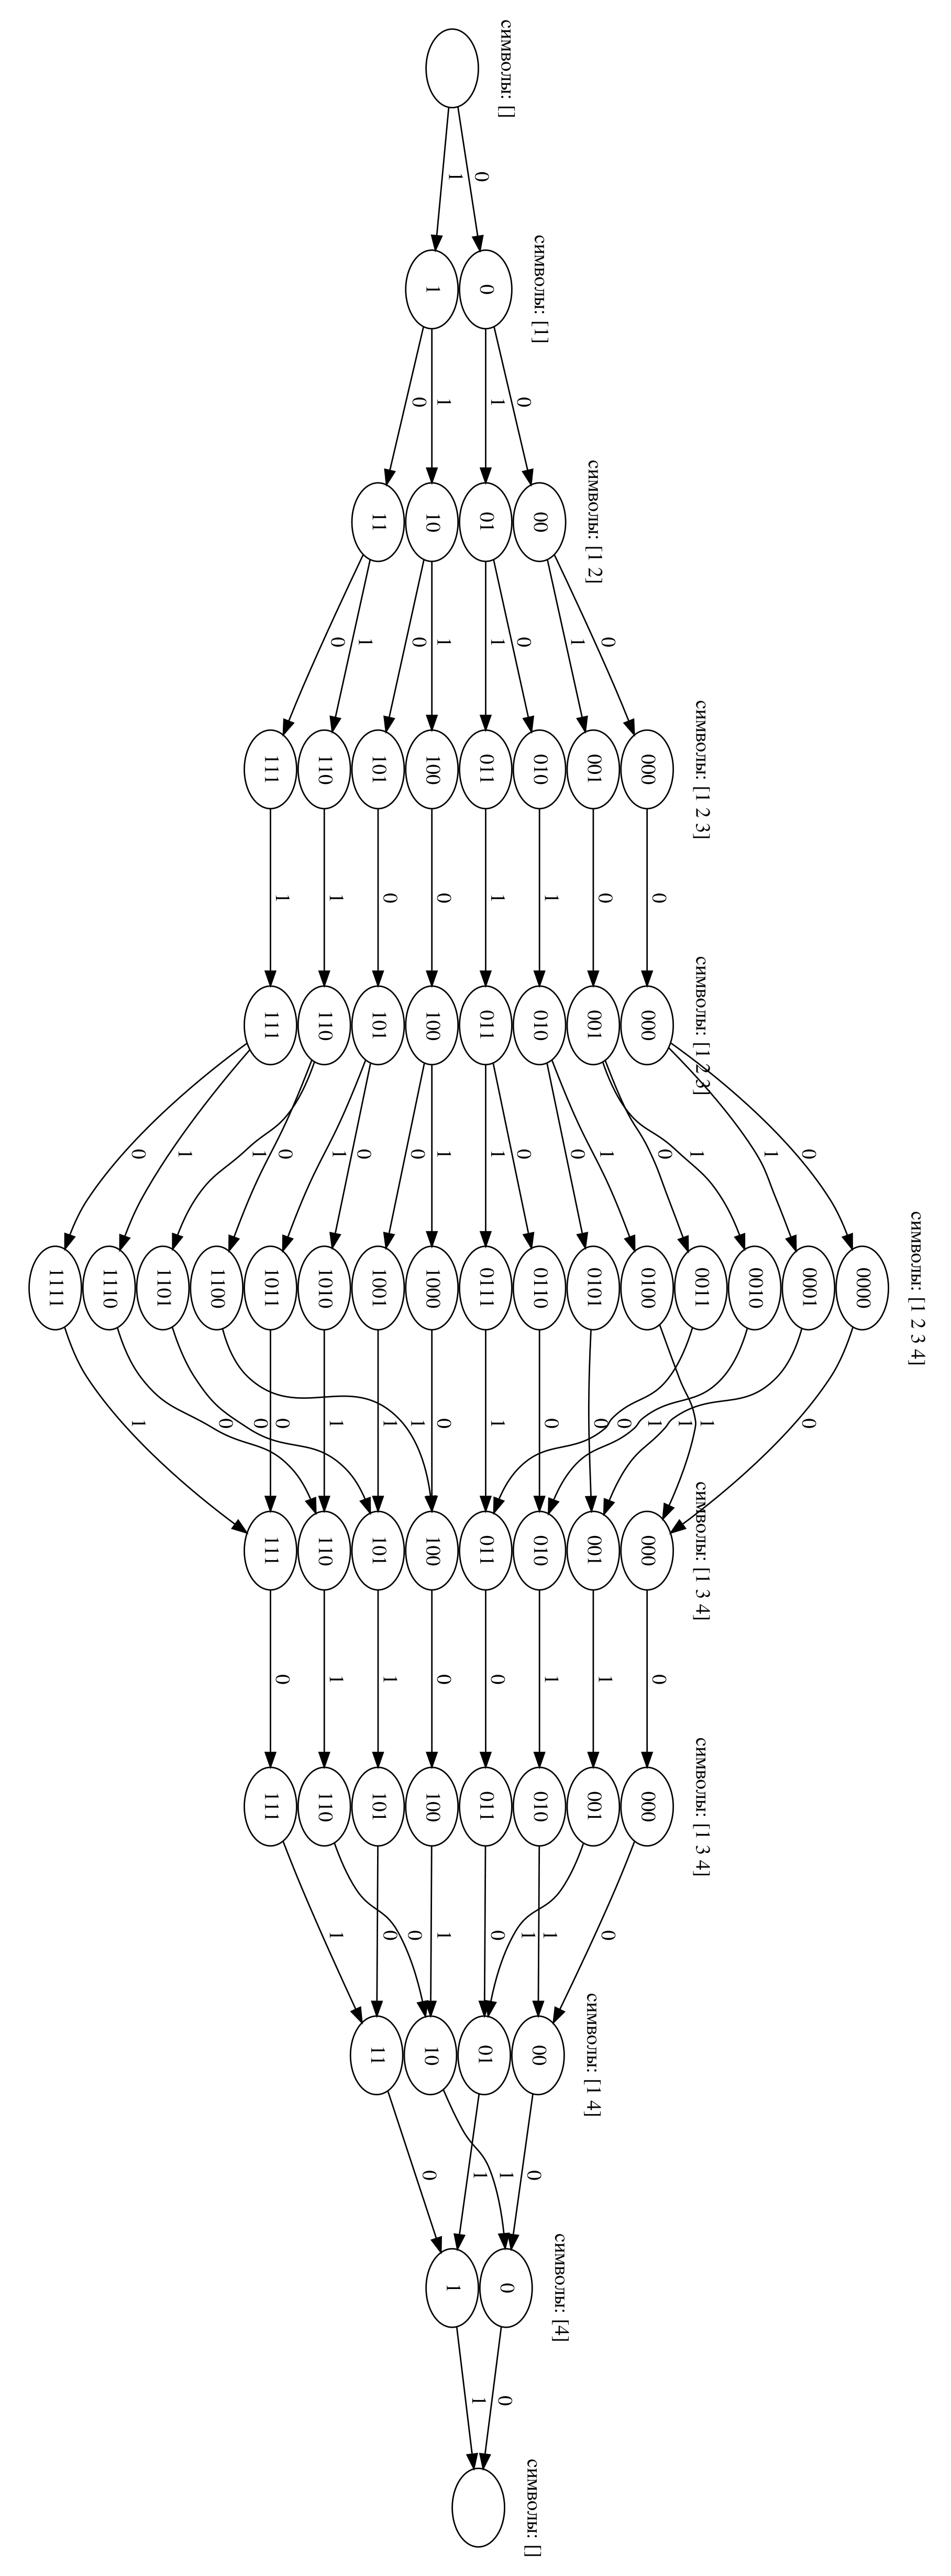
\includegraphics[height=0.95\textheight]{spen.png}
    \caption{Решётка, построенная по МСФ.}
\end{figure}

\end{document}
